% Author: Izaak Neutelings (January 2022)
\documentclass[border=3pt,tikz]{standalone}
\usetikzlibrary{calc}
\usetikzlibrary{intersections}
\usepackage[outline]{contour} % glow around text
\contourlength{0.9pt}

\colorlet{myred}{red!80!black}
\colorlet{myblue}{blue!80!black}
\colorlet{mygreen}{green!80!black}
\colorlet{myorange}{orange!90!black}
\colorlet{mydarkred}{red!60!black}
\colorlet{mydarkblue}{blue!50!black}
\colorlet{mydarkgreen}{green!50!black}
\colorlet{mydarkorange}{orange!70!black}
\newcommand\rightAngle[4]{
  \pgfmathanglebetweenpoints{\pgfpointanchor{#2}{center}}{\pgfpointanchor{#1}{center}}
  \coordinate (tmpRA) at ($(#2)+(\pgfmathresult+45:#4)$);
  \draw[mydarkblue] ($(#2)!(tmpRA)!(#1)$) -- (tmpRA) -- ($(#2)!(tmpRA)!(#3)$);
}
\tikzset{
  angshift/.initial=1,   % shift from origin/center
  angcol/.style={draw=#1!80!black,fill=#1!30}, % shorthand to fill (light) & draw (dark)
  angcol/.default={myblue},
  pics/right angle/.style args={(#1)-(#2)-(#3):#4}{ % right angle
    code={
      \tikzset{angshift/.get=\angshift}
      \pgfmathanglebetweenpoints{\pgfpointanchor{#2}{center}}{\pgfpointanchor{#1}{center}}
      \pgfmathsetmacro\tmpAngA{\pgfmathresult}
      \coordinate (tmpS) at (\tmpAngA+45:\angshift*0.01); % shift
      \coordinate (tmp#1) at ($(#1)+(tmpS)$);
      \coordinate (tmp#2) at ($(#2)+(tmpS)$);
      \coordinate (tmp#3) at ($(#3)+(tmpS)$);
      \coordinate (tmpRA) at ($(tmp#2)+(\tmpAngA+45:#4)$);
      \fill[pic actions,draw=none] % fill square area
        ($(tmp#2)!(tmpRA)!(tmp#1)$) -- (tmpRA) -- ($(tmp#2)!(tmpRA)!(tmp#3)$) -- (tmp#2) -- cycle;
      \draw[pic actions,fill=none] % draw orthogonal mark
        ($(tmp#2)!(tmpRA)!(tmp#1)$) -- (tmpRA) -- ($(tmp#2)!(tmpRA)!(tmp#3)$);
    }
  }
}



\begin{document}


% CYCLIC QUADRILATERAL
% Construct cyclic quadrilateral four points on the circumcircle
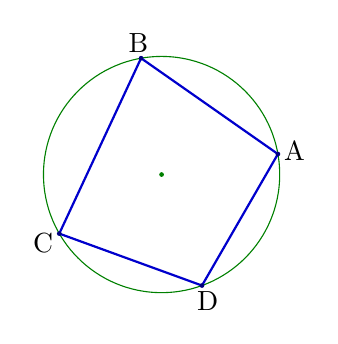
\begin{tikzpicture}[scale=1.5]
  
  \def\R{1.0} % circumradius = radius of circumcircle
  
  % COORDINATES
  \coordinate (O) at (0,0);
  %\coordinate (A) at ( 10:\R);
  %\coordinate (B) at (100:\R);
  %\coordinate (C) at (210:\R);
  %\coordinate (D) at (290:\R);
  \foreach \P/\angP in {A/10,B/100,C/210,D/290}{
    \coordinate (\P) at (\angP:\R); % vertex
    \node[anchor=180+\angP,inner sep=2] at (\P) {\P};
  }
  
  % LINES
  \draw[mydarkgreen] (O) circle(\R);
  \draw[myblue,thick] (A) -- (B) -- (C) -- (D) -- cycle;
  \fill[mydarkgreen] (O) circle(0.02);
  \fill[mydarkblue]
    (A) circle(0.02) (B) circle(0.02)
    (C) circle(0.02) (D) circle(0.02);
  
\end{tikzpicture}


% TANGENTIAL TRAPEZOID
% Construct tangential trapezoid from four points of tangency on the incircle
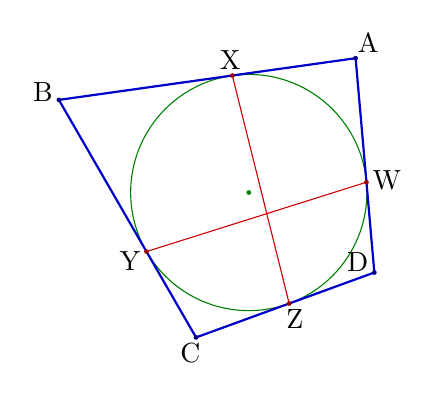
\begin{tikzpicture}[scale=1.5]
  
  \def\R{1.0}  % inradius = radius of incircle
  \def\angW{5} % polar angle of tangent point W
  
  % CIRCLE
  \coordinate (O) at (0,0);
  \draw[mydarkgreen] (O) circle(\R);
  
  % COORDINATES
  \foreach \P/\Q/\angQ [remember={\angQ as \lastang (initially \angW);},
               evaluate={
                 \r=\R/cos((\angQ-\lastang)/2);
                 \angP=(\angQ+\lastang)/2;
               }] in {A/X/98,B/Y/210,C/Z/290,D/W/\angW}{
    \coordinate (\P) at (\angP:\r); % vertex
    \coordinate (\Q) at (\angQ:\R); % point of tangency
    \node[anchor=180+\angP,inner sep=2] at (\P) {\P};
    \node[anchor=180+\angQ,inner sep=2] at (\Q) {\Q};
  }
  
  % LINES
  \draw[myblue,thick] (A) -- (B) -- (C) -- (D) -- cycle;
  \draw[myred] (X) -- (Z) (W) -- (Y);
  \fill[mydarkgreen] (O) circle(0.02);
  \fill[mydarkblue]
    (A) circle(0.02) (B) circle(0.02)
    (C) circle(0.02) (D) circle(0.02);
  \fill[mydarkred]
    (W) circle(0.02) (X) circle(0.02)
    (Y) circle(0.02) (Z) circle(0.02);
  
\end{tikzpicture}


% TANGENTIAL TRAPEZOID using intersections
% Construct tangential trapezoid from four points of tangency on the incircle using intersections
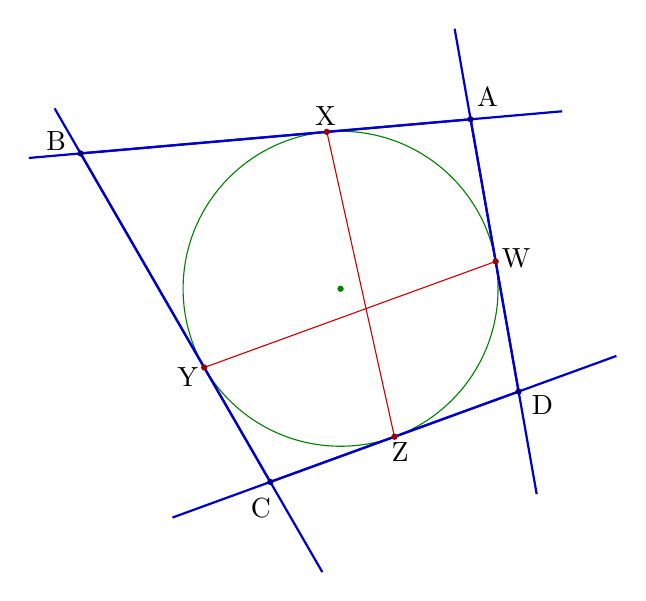
\begin{tikzpicture}[scale=2]
  
  % CIRCLE
  \def\R{1} % inradius = radius of incircle
  \coordinate (O) at (0,0);
  \draw[mydarkgreen] (O) circle(\R);
  
  % COORDINATES
  \foreach \Q/\angQ in {W/10,X/95,Y/210,Z/290}{
    \coordinate (\Q) at (\angQ:\R); % vertex
    \node[anchor=180+\angQ,inner sep=2] at (\Q) {\Q};
  }
  
  % TANGENTS & INTERSECTIONS
  \draw[myblue,thick,name path=W] ($(W)!1.5!90:(O)$) -- (W) -- ($(W)!1.5!-90:(O)$);
  \draw[myblue,thick,name path=X] ($(X)!1.5!90:(O)$) -- (X) -- ($(X)!1.9!-90:(O)$);
  \draw[myblue,thick,name path=Y] ($(Y)!1.9!90:(O)$) -- (Y) -- ($(Y)!1.5!-90:(O)$);
  \draw[myblue,thick,name path=Z] ($(Z)!1.5!90:(O)$) -- (Z) -- ($(Z)!1.5!-90:(O)$);
  \path[name intersections={of={W and X},by=A}] node at ($(A)+(O)!5pt!(A)$) {A};
  \path[name intersections={of={X and Y},by=B}] node at ($(B)+(O)!5pt!(B)$) {B};
  \path[name intersections={of={Y and Z},by=C}] node at ($(C)+(O)!5pt!(C)$) {C};
  \path[name intersections={of={Z and W},by=D}] node at ($(D)+(O)!5pt!(D)$) {D};
  
  % LINES
  \draw[myblue,thick] (A) -- (B) -- (C) -- (D) -- cycle;
  \draw[myred] (X) -- (Z) (W) -- (Y);
  \fill[mydarkgreen] (O) circle(0.02);
  \fill[mydarkblue]
    (A) circle(0.02) (B) circle(0.02)
    (C) circle(0.02) (D) circle(0.02);
  \fill[mydarkred]
    (W) circle(0.02) (X) circle(0.02)
    (Y) circle(0.02) (Z) circle(0.02);
  
\end{tikzpicture}


% BICENTRIC QUADRILATERAL
% http://dynamicmathematicslearning.com/new-bicentric-construction.html
% Construct bicentric quadrilateral for given incircle, circumcircle and one vertex
\foreach \angA in {0,15,40}{ % polar angle of point A
  \foreach \r in {0.55,0.68}{ % inradius = radius of incircle

\begin{tikzpicture}[scale=2.0]
  
  %\def\r{0.68}   % inradius = radius of incircle
  \def\R{1.0}    % circumradius = radius of circumcircle
  \def\angXi{40} % polar angle of incircle center
  %\def\angA{15}  % polar angle of point A
  \pgfmathsetmacro\x{sqrt(\R^2+\r^2-\r*sqrt(4*\R^2+\r^2))} % Fuss's theorem
  
  % CIRCLES
  \coordinate (Oout) at (0,0);
  \coordinate (Oin) at (\angXi:\x);
  \draw[mydarkgreen,line width=0.6] (Oout) -- (Oin)
    node[mydarkgreen!70!black,midway,anchor=\angXi-90,inner sep=1] {$x$};
  \fill[mydarkgreen] (Oin) circle(0.02);
  \fill[mydarkorange] (Oout) circle(0.02);
  \draw[mygreen] (Oin) circle(\r);
  \draw[myorange] (Oout) circle(\R);
  
  % COORDINATES
  \foreach \P/\Q [
    remember={\angP as \lastang (initially \angA);},
    evaluate={
      \d=sqrt(\x^2+\R^2-\r^2-2*\x*\R*cos(\angXi-\lastang));
      \D=sqrt(\d^2+\r^2); %sqrt(\x^2+\R^2-2*\x*\R*cos(\angXi-\lastang));
      \tanang=90+atan2(\d,\r)+atan2(\R*sin(\lastang)-\x*sin(\angXi),\R*cos(\lastang)-\x*cos(\angXi));
      \angP=2*\tanang-\lastang-180;
    }] in {B/W,C/X,D/Y,A/Z}{
    \coordinate (\P) at (\angP:\R); % corner
    \coordinate (\Q) at ($(\lastang:\R)+(\tanang:\d)$); % point of tangency
    \node[mydarkblue!80!black,anchor=180+\angP,inner sep=2] at (\P) {\P};
    \node[mydarkred!80!black,anchor=90+\tanang,inner sep=2] at (\Q) {\Q};
  }
  \coordinate (A) at (\angA:\R); % overwrite for precision
  
  % SIDES
  \draw[myblue,thick] (A) -- (B) -- (C) -- (D) -- cycle;
  \draw[myred,name path=a] (X) -- (Z);
  \draw[myred,name path=b] (W) -- (Y);
  \fill[mydarkblue]
    (A) circle(0.02) (B) circle(0.02)
    (C) circle(0.02) (D) circle(0.02);
  \fill[mydarkred]
    (W) circle(0.02) (X) circle(0.02)
    (Y) circle(0.02) (Z) circle(0.02);
  \path[name intersections={of={a and b},by=C}]; % get intersection C
  \rightAngle{Z}{C}{W}{0.15} % mark right angle
  
\end{tikzpicture}
  }
}


% BICENTRIC QUADRILATERAL - right kite
% https://en.wikipedia.org/wiki/Right_kite
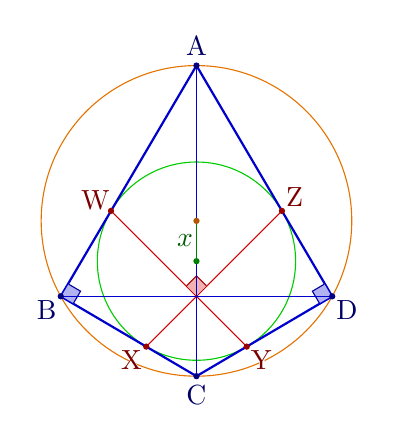
\begin{tikzpicture}[scale=2.0]
  
  \def\a{1.7} % length of long sides
  \def\b{1.0} % length of short sides
  \pgfmathsetmacro\angA{2*atan2(\b,\a)} % angle A = B--A--D
  \pgfmathsetmacro\angC{180-\angA}      % angle C = B--C--D
  \pgfmathsetmacro\R{sqrt(\a^2+\b^2)/2} % circumradius = radius of circumcircle
  \pgfmathsetmacro\r{\a*\b/(\a+\b)}     % inradius = radius of incircle
  \pgfmathsetmacro\R{sqrt(\a^2+\b^2)/2} % Fuss's theorem
  \pgfmathsetmacro\x{sqrt(\R^2+\r^2-\r*sqrt(4*\R^2+\r^2))} % Fuss's theorem
  
  % COORDINATES
  \coordinate (Oout) at (0,0);
  \coordinate (Oin) at (-90:\x);
  \coordinate (A) at (90:\R);
  \coordinate (B) at (270-\angA:\R);
  \coordinate (C) at (-90:\R);
  \coordinate (D) at (\angA-90:\R);
  \coordinate (W) at ($(Oin)+(180-\angA/2:\r)$);
  \coordinate (X) at ($(Oin)+(180+\angC/2:\r)$);
  \coordinate (Y) at ($(Oin)+(-\angC/2:\r)$);
  \coordinate (Z) at ($(Oin)+(\angA/2:\r)$);
  
  % CIRCLES
  \draw[mygreen] (Oin) circle(\r);
  \draw[myorange] (Oout) circle(\R);
  
  % SIDES
  \draw[myblue,thick] (A) -- (B) -- (C) -- (D) -- cycle;
  \draw[myred,name path=a] (X) -- (Z);
  \draw[myred,name path=b] (W) -- (Y);
    
  % MARK ANGLES
  \path[name intersections={of={a and b},by=O}]; % get intersection O
  %\rightAngle{Z}{C}{W}{0.15} % mark right angle
  %\rightAngle{X}{B}{W}{0.15} % mark right angle
  %\rightAngle{Z}{D}{Y}{0.15} % mark right angle
  \pic[angcol=myred] {right angle={(Z)-(O)-(W):0.25}};
  \pic[angcol=myblue] {right angle={(X)-(B)-(W):0.25}};
  \pic[angcol=myblue] {right angle={(Z)-(D)-(Y):0.25}};
  \draw[myblue,thin] (A) -- (C) (B) -- (D);
  \draw[mydarkgreen,thick,line width=0.6] (Oout) -- (Oin)
    node[mydarkgreen!70!black,midway,anchor=0,inner sep=1] {$x$};
  
  % DOTS
  \fill[mydarkgreen] (Oin) circle(0.02);
  \fill[mydarkorange] (Oout) circle(0.02);
  \fill[mydarkblue]
    (A) circle(0.02) node[mydarkblue!80!black,above] {A}
    (B) circle(0.02) node[mydarkblue!80!black,below left=-2] {B}
    (C) circle(0.02) node[mydarkblue!80!black,below] {C}
    (D) circle(0.02) node[mydarkblue!80!black,below right=-2] {D};
  \fill[mydarkred]
    (W) circle(0.02) node[mydarkred!80!black,above left=-3] {W}
    (X) circle(0.02) node[mydarkred!80!black,below left=-2] {\contour{white}{X}}
    (Y) circle(0.02) node[mydarkred!80!black,below right=-2] {\contour{white}{Y}}
    (Z) circle(0.02) node[mydarkred!80!black,above right=-2] {Z};
  
\end{tikzpicture}


\end{document}